\section{Problem 2}\label{prob2}

The global snapshot need not be consistent. Below, we provide a counterexample to demonstrate the inconsistency in the global snapshot.

Consider a system with three nodes: \(A\), \(B\), and \(C\), connected by three bidirectional communication links: \(AB\), \(BC\), and \(AC\). Assume the presence of an external reference clock used only for reference purposes, which does not interfere with the system.

Assume the following clock synchronization properties:
- Nodes \(B\) and \(C\) are perfectly synchronized with the reference clock.
- Node \(A\) runs 1 second slower than the reference clock. Specifically, if the reference clock shows time \(x\), the clocks of \(B\) and \(C\) also show \(x\), while the clock of \(A\) shows \(x - 1\).(in seconds)

This assumption aligns with the problem statement, which specifies that the clocks of all three nodes are synchronized to within 1 second of each other.

\begin{figure}[h]
    \centering
    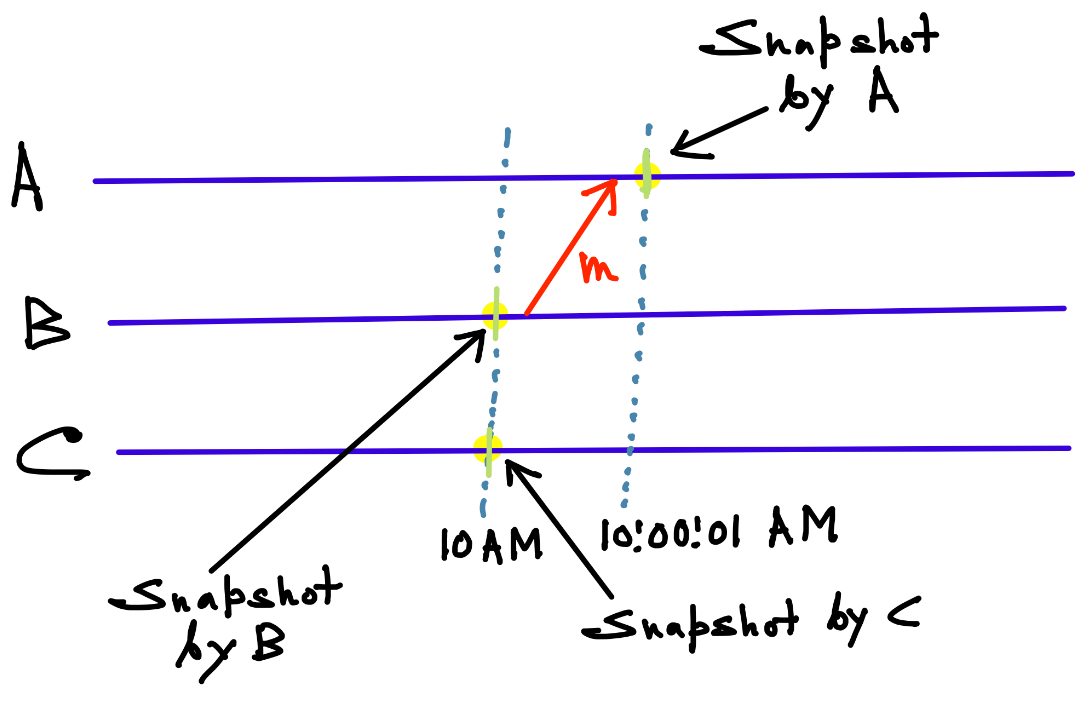
\includegraphics[width=0.5\textwidth]{IMG/Q2.jpeg}
    \caption{Timeline of Events}
    \label{fig:timeline}
\end{figure}

Let us analyze the snapshot operation at the reference time \(10{:}00{:}00\):  
\begin{itemize}
    \item At this time, the clock of node \(A\) displays \(09{:}59{:}59\).  
    \item The clocks of nodes \(B\) and \(C\) both display \(10{:}00{:}00\).  
\end{itemize}

Nodes \(B\) and \(C\) store their snapshots immediately at \(10{:}00{:}00\) (reference clock), whereas node \(A\) stores its snapshot when its clock reaches \(10{:}00{:}00\), which corresponds to the reference time \(10{:}00{:}01\).

Now, consider the following message-passing scenario:  
\begin{itemize}
    \item Node \(B\) sends a message \(m\) to node \(A\) just after the reference time \(10{:}00{:}00\).  
    \item Node \(A\) receives this message just before its clock reaches \(10{:}00{:}00\) (at reference time \(10{:}00{:}01\)).  
\end{itemize}

In this case:  
\begin{itemize}
    \item In the snapshot recorded by \(B\), the send event of message \(m\) will not be recorded. That is, \(\texttt{send}(m) \notin LS_B\).
    \item In the snapshot recorded by \(A\), the receive event of message \(m\) will be recorded. That is, \(\texttt{receive}(m) \in LS_A\).
\end{itemize}

Thus, the global snapshot will contain an inconsistency:  
\[
\texttt{inconsistent}(LS_B, LS_A) = \{m\}
\]
Since this set is not empty, the global snapshot is inconsistent.
